\section{Synchronizing the time}

Because the clients may run on different computers the computer clock time cannot be used as a parameter to the animations since the computer clocks are unlikely to be in sync with each other. As shown in chapter 1 this is a well known problem in distributed systems, so the first step would be to implement one or several existing synchronization algorithms. 

A combination of the Berkley algoritm described in \ref{sec:berkley} and NTP described in \ref{sec:ntp} was used to synchronize the time of the clients and the server. Both NTP and the Berkley algorithm are designed to be used in intranets since they assume an evenly distributed delay. The end product that the work in this thesis is intended to be used in is assumed to run on an intranet. The accuracy given by these algoritms is assumed to be good enough. 

An artificial time is created both on the server and on the clients on start and this time is never manipulated. Instead a delta value added to the artificial time is used as input to the animations.  

\subsection {Distributing deltas}

The server initiates the synchronization with the clients by sending a sync event message to the clients. The clients reply with the time they recieved the message, the time they send their reply and their old delta-value. The server then calculates each clients delta and sends each client a message containing their new delta. 

If the value of the old delta of the client and the new delta calculated by the server differs more than 2 milliseconds the server will send a new sync event as a message to the client, repeating the procedure until the delta is stable. 

Every time a new client connects to the server this client needs to synchronize its time with the server's. 

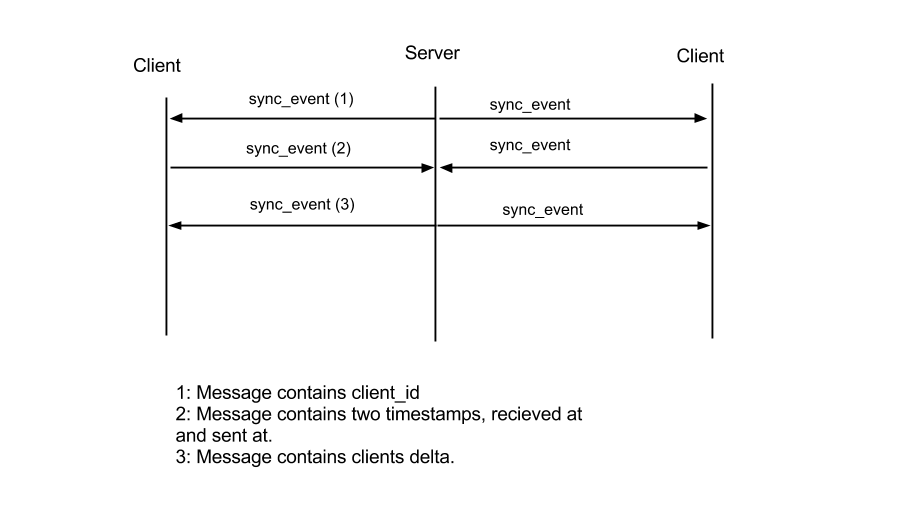
\includegraphics[width=1.0\textwidth]{figures/comm.png}

\subsection{Calculating deltas}
An implementation of NTP was used to calculate each clients latency, shown below. This calculation is done on the server and the delta value calculated is the NTP master offset. 

\begin{verbatim}
self.delta = ((self.t_1 - self.t_0) + (self.t_2 - self.t_3))/2
\end{verbatim}

\subsection {Using the delta values}

All animations must take a timestamp as a parameter for playback. This is used to timestep through the animation. To create the timestamp the client uses the time acquired when the delta is added to its own local time. This way all client's animations will be synchronized, they will be at the same stage in the animation at the same time given that they have their correct delta value. 


